% ============================================================
%  Figure 11 — RMS residual vs window length
% ============================================================
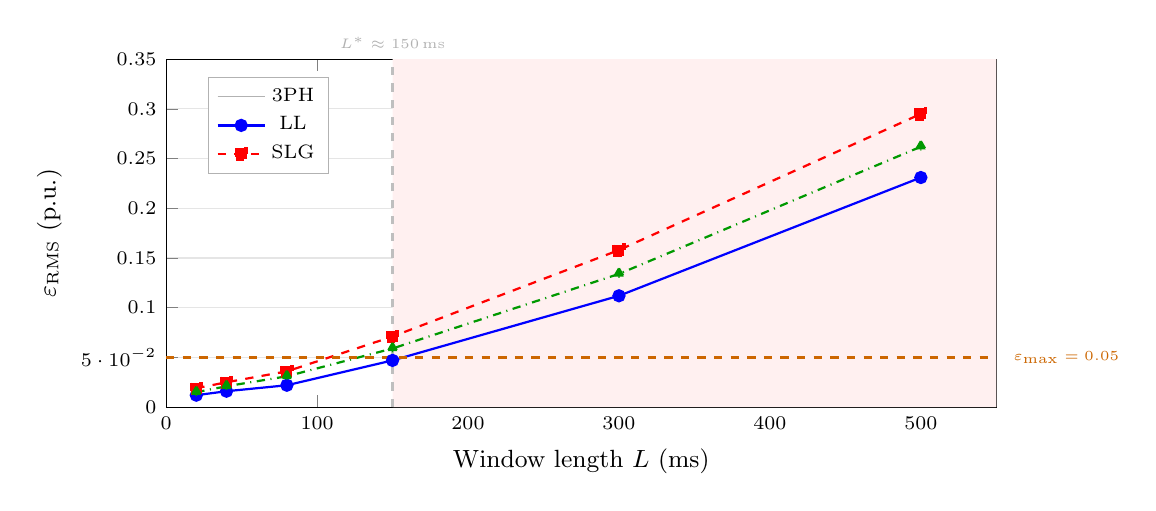
\begin{tikzpicture}
\begin{axis}[
  width=\columnwidth, height=6.0cm,
  xlabel={Window length $L$ (ms)},
  ylabel={$\varepsilon_{\mathrm{RMS}}$ (p.u.)},
  xmin=0, xmax=550, ymin=0, ymax=0.35,
  xtick={0,100,200,300,400,500},
  ytick={0,0.05,0.10,0.15,0.20,0.25,0.30,0.35},
  ymajorgrids=true, grid style={gray!20},
  label style={font=\small},
  tick label style={font=\scriptsize},
  legend style={at={(0.05,0.95)}, anchor=north west,
                font=\scriptsize, fill=white, draw=black!30},
  clip=false
]

% Shaded invalid region L > 150ms
\addplot[fill=red!6, draw=none]
  coordinates {(150,0)(550,0)(550,0.35)(150,0.35)} \closedcycle;

% 3PH
\addplot[blue, solid, thick, mark=*, mark size=2pt] coordinates {
  (20,0.012)(40,0.016)(80,0.022)(150,0.047)(300,0.112)(500,0.231)
};

% LL
\addplot[red, dashed, thick, mark=square*, mark size=2pt] coordinates {
  (20,0.019)(40,0.025)(80,0.036)(150,0.071)(300,0.158)(500,0.295)
};

% SLG
\addplot[green!60!black, dashdotted, thick, mark=triangle*, mark size=2pt] coordinates {
  (20,0.015)(40,0.021)(80,0.031)(150,0.059)(300,0.134)(500,0.262)
};

% Acceptance threshold
\draw[thick, orange!80!black, dashed]
     (axis cs:0, 0.05) -- (axis cs:550, 0.05);
\node[right, font=\tiny, orange!80!black]
     at (axis cs:555, 0.05) {$\varepsilon_{\max}=0.05$};

% Validity boundary
\draw[thick, gray!50, dashed]
     (axis cs:150, 0) -- (axis cs:150, 0.35);
\node[above, font=\tiny, gray!60] at (axis cs:150, 0.35) {$L^*\approx 150$\,ms};

\legend{3PH, LL, SLG};

\end{axis}
\end{tikzpicture}
